\documentclass[letter]{article}
\usepackage[monocolor]{../math232/ahsansabit}
\usepackage[]{float}
\usepackage[]{pgfplots}\title{Quantum Mechanics : : Homework 04}
\author{Ahmed Saad Sabit, Rice University}
\date{\today}

\begin{document}
\maketitle


\section*{Problem 01}
\subsection*{a} 
I do the matrix multiplication by hand. 
\begin{align*}
	\hat{\sigma}_1 \hat{\sigma}_2  &= \begin{pmatrix} 0&1\\1&0 \end{pmatrix} 
	\begin{pmatrix} 0&-i\\i&0 \end{pmatrix}  =
	\begin{pmatrix} i&0\\0&-i \end{pmatrix} = i \hat{\sigma}_3 \\ 
	\hat{\sigma}_2 \hat{\sigma}_1 &= \begin{pmatrix} 0&-i\\i&0 \end{pmatrix} 
	\begin{pmatrix} 0&1\\1&0 \end{pmatrix} = \begin{pmatrix} -i&0\\0&i \end{pmatrix} = - i \hat{\sigma}_3 \\
	\hat{\sigma_2}\hat{\sigma}_3 &= \begin{pmatrix} 0&-i\\i&0 \end{pmatrix} 
	\begin{pmatrix} 1&0\\0&-1 \end{pmatrix} = 
	\begin{pmatrix} 0&i\\i&0 \end{pmatrix} = i \hat{\sigma}_1
	\\ \hat{\sigma_3}\hat{\sigma}_2 &= 	\begin{pmatrix} 1&0\\0&-1 \end{pmatrix}  
	\begin{pmatrix} 0&-i\\i&0 \end{pmatrix} = 
\begin{pmatrix} 0&-i\\-i&0 \end{pmatrix} = -i \hat{\sigma}_1 \\ 
\hat{\sigma}_3 \hat{\sigma}_1  &= 
\begin{pmatrix} 1&0\\0&-1  \end{pmatrix} 
\begin{pmatrix} 0&1\\1&0 \end{pmatrix} 
= \begin{pmatrix} 0&1\\-1&0 \end{pmatrix}  = i \hat{\sigma}_2 \\ 
\hat{\sigma}_1 \hat{\sigma}_3  &= 
\begin{pmatrix} 0&1\\1&0 \end{pmatrix} 
\begin{pmatrix} 1&0\\0&-1  \end{pmatrix} 
= \begin{pmatrix} 0&-1\\1&0 \end{pmatrix}  = -i \hat{\sigma}_2 \\ 
\end{align*}
The cross product 
\begin{align*}
	\hat{\vec{\sigma}} \times \hat{\vec{\sigma}} 
&= \begin{vmatrix} \vec{n}_x & \vec{n}_y & \vec{n}_z \\
\sigma_1 & \sigma_2 & \sigma_3 \\ 
\sigma_1 & \sigma_2 & \sigma_3 \\ 
\end{vmatrix}  \\
	&= \vec{n}_x \left(\sigma_2 \sigma_3 - \sigma_3 \sigma_2\right) + \vec{n}_y \left(\sigma_3 \sigma_1 - \sigma_1 \sigma_3 \right) + \vec{n}_z \left(\sigma_1 \sigma_2 - \sigma_2 \sigma_1\right)  \\ 
	&= \vec{n}_x (2 i \sigma_1) + \vec{n}_y \left( 2 i \sigma_2\right) + \vec{n}_z \left(2 i \sigma_3\right) \\
	&= 2 i \left(\sigma_1 \vec{n}_x + \sigma_2 \vec{n}_y + \sigma_3 \vec{n}_z\right) \\
	&= 2 i \hat{\vec{\sigma}} \\
\end{align*}
Note this also is alluring to the Levi-Civita Symbol because 
\[ \text{cyclic }
i \to j \to k \to i \to j \to  k \implies
	\quad \sigma_i \sigma_j = i\epsilon_{ij} \sigma_k \tag{where $\{i,j,k\} \in \{1,2,3\} $ }
\]



\subsection*{b} 
\begin{align*}
	\left(\vec{U} \cdot  \hat{\vec{\sigma}}\right) 
	\left(\vec{V} \cdot  \hat{\vec{\sigma}}\right) &= 
	\left(U_1 \sigma_1 + U_2 \sigma_2 + U_3 \sigma_3\right)
	\left(V_1 \sigma_1 + V_2 \sigma_2 + V_3 \sigma_3\right)\\
\end{align*}

\begin{align*}
	\left(\vec{U} \cdot \hat{\vec{\sigma}}\right)
	\left(\vec{V}\cdot \hat{\vec{\sigma}}\right) &= 
	\left(\sum_{i= 1}^{3} U_i \sigma_i\right)
	\left(\sum_{j=1}^{3} V_j \sigma_j\right) \\
	&= 
\sum_{i,j = 1}^{3} U_i V_j \sigma_i \sigma_j
	\\
	&= 
\sum_{i,j = 1, i\neq j}^{3} U_i V_j \sigma_i \sigma_j + \sum_{n=1}^{3} U_n V_n \sigma_n \sigma_n 
	\\ 
	&= 
	\sum_{i,j = 1, i\neq j}^{3} i U_i V_j \epsilon_{ij} \sigma_k + \sum_{n=1}^{3} U_n V_n \sigma_n \sigma_n 
	\\ 
	&= \left[  i(U_1 V_2 - U_2 V_1) \sigma_3 + i (U_2 U_3 - U_3 U_2) \sigma_1 + i (U_3 U_1 - U_1 U_3) \sigma_2  \right] + (U_1 V_1 + U_2 V_2 + U_3 V_3) \hat{I} \\ 
	&= [ \vec{U} \times  \vec{V}]_3 i \sigma_3 + [ \vec{U} \times \vec{V}]_1 i \sigma_1 + 
	[\vec{U} \times  \vec{V}]_2 i \sigma_2 + (\vec{U} \cdot \vec{V}) \hat{I}\\
	&= i \left[ \vec{U} \times \vec{V}\right] \cdot \hat{\vec{\sigma}} + \left(\vec{U}\cdot \vec{V}\right) \hat{I} \\
\end{align*}



\newpage
\section*{Problem 02}
\subsection*{a} 
Considering the simplest basis in column vector forms 
\[
| 1 \rangle = \begin{pmatrix} 1\\0\\0 \end{pmatrix} 
\quad
| 2 \rangle = \begin{pmatrix} 0\\1\\0 \end{pmatrix} 
\quad
| 3 \rangle = \begin{pmatrix} 0\\0\\1 \end{pmatrix} 
\] 
We want to compute the following operator $\hat{H}$ 
\begin{align*}
	\hat{H}= 
	E_0\left(
	| 1 \rangle \langle 1 |  + | 2 \rangle \langle 2 |  + | 3 \rangle \langle 3 | 
	\right) - J
	\left(
	| 1 \rangle \langle 2 | + | 2 \rangle \langle 1  | +
	| 2 \rangle \langle 3 | + | 3 \rangle \langle 2 | + 
	| 3 \rangle \langle 1 | + | 1 \rangle \langle 3 |  
	\right) 
\end{align*}
Matrices for the first term
\begin{align*}
	| 1 \rangle \langle 1 |  + | 2 \rangle \langle 2 |  + | 3 \rangle \langle 3 |  &
= \begin{bmatrix} 1\\0\\0 \end{bmatrix} \begin{bmatrix} 1&0&0 \end{bmatrix} + 
\begin{bmatrix} 0\\1\\0 \end{bmatrix} \begin{bmatrix} 0&1&0 \end{bmatrix} + 
\begin{bmatrix} 0\\0\\1 \end{bmatrix} \begin{bmatrix} 0&0&1 \end{bmatrix} \\ 
						       & =
\begin{pmatrix} 1&0&0\\0&0&0\\0&0&0 \end{pmatrix} +
\begin{pmatrix} 0&0&0\\0&1&0\\0&0&0 \end{pmatrix} + 
\begin{pmatrix} 0&0&0\\0&0&0\\0&0&1 \end{pmatrix} \\  
		 &= \begin{pmatrix} 1&0&0\\0&1&0\\0&0&1 \end{pmatrix} = \hat{I} 
\end{align*}

Matrices for the second term 
\begin{align*}
&	| 1 \rangle \langle 2 | + | 2 \rangle \langle 1  | +
	| 2 \rangle \langle 3 | + | 3 \rangle \langle 2 | + 
	| 3 \rangle \langle 1 | + | 1 \rangle \langle 3 |  \\ 
	&= 
	\begin{pmatrix} 1\\0\\0 \end{pmatrix} \begin{pmatrix} 0&1&0 \end{pmatrix} +
	\begin{pmatrix} 0\\1\\0 \end{pmatrix} \begin{pmatrix} 1&0&0 \end{pmatrix}  +
	\begin{pmatrix} 0\\1\\0 \end{pmatrix} \begin{pmatrix} 0&0&1 \end{pmatrix} + 
	\begin{pmatrix} 0\\0\\1 \end{pmatrix} \begin{pmatrix} 0&1&0 \end{pmatrix} + 
	\begin{pmatrix} 0\\0\\1 \end{pmatrix} \begin{pmatrix} 1&0&0 \end{pmatrix} + 
	\begin{pmatrix} 1\\0\\0 \end{pmatrix} \begin{pmatrix} 0&0&1 \end{pmatrix} 
	\\
	&= 
	\begin{bmatrix} 0&1&0\\0&0&0\\0&0&0 \end{bmatrix} + 
	\begin{bmatrix} 0&0&0\\1&0&0\\0&0&0 \end{bmatrix} +
	\begin{bmatrix} 0&0&0\\0&0&1\\0&0&0 \end{bmatrix} + 
	\begin{bmatrix} 0&0&0\\0&0&0\\0&1&0 \end{bmatrix} + 
	\begin{bmatrix} 0&0&0\\0&0&0\\1&0&0 \end{bmatrix} + 
	\begin{bmatrix} 0&0&1\\0&0&0\\0&0&0 \end{bmatrix} 
	\\
	&= 
	\begin{bmatrix} 0&1&1\\1&0&1\\1&1&0 \end{bmatrix} 
	\\
\end{align*}

Put them all together 
\begin{align*}
	\hat{H} &= 
	E_0\left(
	| 1 \rangle \langle 1 |  + | 2 \rangle \langle 2 |  + | 3 \rangle \langle 3 | 
	\right) - J
	\left(
	| 1 \rangle \langle 2 | + | 2 \rangle \langle 1  | +
	| 2 \rangle \langle 3 | + | 3 \rangle \langle 2 | + 
	| 3 \rangle \langle 1 | + | 1 \rangle \langle 3 |  
	\right) \\ 
		&= \begin{bmatrix} E_0&-J&-J\\-J&E_0&-J\\-J&-J&E_0 \end{bmatrix}  \\
\end{align*}




\subsection*{b (i)} 
The $| E_1 \rangle $ in column vector representation 
\[
| E_1 \rangle  = \frac{1}{\sqrt{3} } \left(| 1 \rangle + | 2 \rangle + | 3 \rangle \right) = 
	\frac{1}{\sqrt{3} } \begin{bmatrix} 1\\1\\1 \end{bmatrix}  
\]

Computing $\hat{H} | E_1 \rangle $
\begin{align*}
	\hat{H} | E_1 \rangle  &=  
	\begin{bmatrix} E_0&-J&-J\\-J&E_0&-J\\-J&-J&E_0 \end{bmatrix} 
	\left(
\frac{1}{\sqrt{3} } \begin{bmatrix} 1\\1\\1 \end{bmatrix} 
	\right)
	\\
	&= 
\frac{1}{\sqrt{3} } 
\begin{bmatrix} E_0 - J - J \\ -J + E_0 - J \\ - J - J + E_0  \end{bmatrix} 
	\\
	&= 
\frac{1}{\sqrt{3} } 
\begin{bmatrix} E_0 - 2J \\ E_0 - 2 J \\ E_0 - 2J  \end{bmatrix} 
	\\ 
	&= \frac{E_0 - 2J}{\sqrt{3} } \begin{bmatrix} 1\\1\\1 \end{bmatrix}  \\
	&= \left(E_0 - 2J\right) | E_1 \rangle  
\end{align*}
We see the eigen-equation for the Hamiltonian 
\[
\hat{H} | E_1 \rangle  = E_1 | E_1 \rangle  \implies E_1 = E_0 - 2J
\] 


The special property can be realized by seeing that,
\begin{align*}
	\begin{bmatrix} E_0&-J&-J\\-J&E_0&-J\\-J&-J&E_0 \end{bmatrix}  &= 
	(E_0 + J)\begin{bmatrix}  1 &0&0\\0&1&0\\0&0&1 \end{bmatrix}  + 
	(-J) \begin{bmatrix} 1&1&1\\1&1&1\\1&1&1 \end{bmatrix} 
	\\
\end{align*}
It's very obvious that $| E_1 \rangle $ is an eigenvector for both of the upper matrices. And if $\hat{H} = \hat{A} + \hat{B}$ then if $| E_1 \rangle $ is eigenvector for both $\hat{A},\hat{B}$, then 
\[ \hat{H} | E_1 \rangle =
\hat{A} | E_1 \rangle + \hat{B} | E_1 \rangle  = (a+b)| E_1 \rangle = E_1 | E_1 \rangle 
\]
Just from looking at the matrices it's obvious that $a = E_0+J$ and $b = -3J$ so $E_1 = E_0 - 2J$


\subsection*{b (ii) and (iii)} 
We algebraically initialize the elements of the matrix to minimize the computational effort by hand. Keep in mind that $\hat{H} - E \hat{I } = \hat{0} = \frac{1}{J} \hat{H} - \frac{1}{J} E \hat{I} $ hence 
\begin{align*}
	\frac{1}{J} \hat{H} &= 
	\begin{bmatrix} \frac{E_0}{J} & -1 & -1 \\ -1 &  \frac{E_0}{J} & -1 \\ 
	-1 & -1 &  \frac{E_0}{J}\end{bmatrix}  
	\\
		\left(\frac{1}{J} \hat{H}\right) - \frac{E}{J} \hat{I} &=
	\begin{bmatrix} \frac{E_0 - E}{J} & -1 & -1 \\ -1 &  \frac{E_0 - E}{J} & -1 \\ 
	-1 & -1 &  \frac{E_0 - E}{J}\end{bmatrix}   \\ 
					  &= (-1) \begin{bmatrix} \lambda & 1 & 1 \\ 
					  1 & \lambda & 1 \\ 1 & 1 & \lambda \end{bmatrix} \tag{$\lambda = (E - E_0 )/ J$}  = 0  \\ 
					  & \implies \det  
					   \begin{bmatrix} \lambda & 1 & 1 \\ 
					  1 & \lambda & 1 \\ 1 & 1 & \lambda \end{bmatrix}  = 0\\  
								   & \implies \lambda^3 + 3 \lambda + 2 = 0  \\ 
								   & \implies ( \lambda - 1)^2 (\lambda + 2) = 0 \\
& \implies (\lambda^2 - 2 \lambda + 1 ) (\lambda + 2 ) \\ 
	& \implies \lambda = 1, 1, -2 
\end{align*}
As stated in the problem statement, $0 = (\lambda - \lambda_1 ) (\lambda^2 + b \lambda + c) \implies 0 = (\lambda - (-2)) (\lambda^2 + (-2) \lambda + 1  )$ giving us $(b,c) = (-2, 1)$
\[
	\text{For } \lambda = -2 \text{ the eigen-energy is } \frac{E - E_0}{J} = -2 \implies E = E_0 - 2 J  
\] 
\[
	\text{For } \lambda = 1 \text{ the eigen-energy is } \frac{E - E_0}{J} = 1 \implies E = E_0 +  J  
\]
The eigenvalues are 
\[
\lambda_1 = -2, \quad \lambda_2 = 1, \quad \lambda_3 = 1
\]
And corresponding eigen-energy
\[
E_1 = E_0 - 2 J , \quad E_2 = E_0+ J , \quad E_3 = E_0 + J
\] 

\newpage
\section*{Problem 03} 

\subsection*{a} 
\begin{align*}
	\hat{T} | n \rangle  = | n+1 \rangle  &\implies \langle n | T^\dagger = \langle n+1 | \\ 
					      &\text{now, } \langle n | T^\dagger | n+1 \rangle = 
					      \langle n+1 | | n+1 \rangle  = 1 \\ 
					      &\text{or, } 
					      \langle n | T^\dagger T | n \rangle = 1 \\  
					      &\text{and, } \langle n | T^\dagger | k+1 \rangle = 
					      \langle n+1| | k+1 \rangle \tag{$n\neq k$ } = 0 
					   \\ & \implies T^\dagger T = \hat{I}
\end{align*}


\subsection*{b}
To compute $\left[ \hat{H}, \hat{T} \right] $ we compute the two operator terms individually
\begin{align*}
	\hat{H} \hat{T} &= 
\left(
	%
\sum_{n=-\infty}^{\infty} 
\left[
E_0 | n \rangle \langle n | + 
J 
\left(
| n+1 \rangle \langle n | + 
| n \rangle \langle n+1 | 
\right)
\right] 
%
\right) 
\hat{T} 
\\ \hat{H} \hat{T} | n \rangle  &= 
\left(
	%
\sum_{n=-\infty}^{\infty} 
\left[
E_0 | n \rangle \langle n | + 
J 
\left(
| n+1 \rangle \langle n | + 
| n \rangle \langle n+1 | 
\right)
\right] 
%
\right)  | n+1 \rangle 
\\ 
&= 
\Bigl[
E_0 | n \rangle  \langle n | + 
J \Bigl(
| n+1 \rangle \langle n | + 
| n \rangle \langle n+1 | 
\Bigr)
\Bigr] | n+1 \rangle  + 
%
\Bigl[
E_0 | n+1 \rangle \langle n+1 | + 
J \Bigl(
| n+2 \rangle \langle n+1 | + 
| n+1 \rangle \langle n+2 | 
\Bigr)
\Bigr] | n+1 \rangle  
\\
&= 
J | n \rangle + 
E_0 | n + 1\rangle  + 
J 
\left(
| n+2 \rangle 
\right)
\\
\hat{T}\hat{H} | n \rangle  &= 
\hat{T}\Biggr(
\Bigl[
E_0 | n \rangle  \langle n | + 
J \Bigl(
| n+1 \rangle \langle n | + 
| n \rangle \langle n+1 | 
\Bigr)
\Bigr] | n \rangle  + 
%
\Bigl[
E_0 | n-1 \rangle \langle n-1 | + 
J
\Bigl(
| n \rangle \langle n-1 | + | n-1 \rangle \langle n | 
	\Bigr)
\Bigr] | n \rangle 
\Biggr) \\ 
&= 
\hat{T} \bigl(
E_0 | n \rangle + J | n+1 \rangle + J | n-1 \rangle 
\bigr) \\ 
&= E_0 | n+1 \rangle + J | n+2 \rangle + J | n \rangle  = \hat{H} \hat{T} | n \rangle \\
\end{align*} 
\[
\therefore \left(\hat{H}\hat{T} - \hat{T}\hat{H}\right) | n \rangle  = | 0 \rangle  \implies
\left[
	\hat{H}, \hat{T} 
\right] = 0
\] 


\subsection*{c} 
Using the form given for the energy, and the eigen-equation for $\hat{T}$, we determine the general formula for $\psi_{E,n}$ in terms of $\psi_{E,0}$
\begin{align*}
	| E \rangle  &= \sum_{n=-\infty}^{\infty} | n \rangle \psi_{E,n} \\ 
	T | E \rangle  &= \sum_{n=-\infty}^{\infty} T | n \rangle \psi_{E,n}\\ 
	e^{-i \phi} | E \rangle 	       &= \sum_{n=-\infty}^{\infty} | n+1 \rangle \psi_{E,n} \\ 
	\sum_{n=-\infty}^{\infty} e^{-i \phi} | n \rangle \psi_{E,n} &= \sum_{n=-\infty}^{\infty} | n+1 \rangle \psi_{E,n} \\ 
	\implies e^{-i \phi} | n+1 \rangle \psi_{E,n+1} &= | n+1 \rangle \psi_{E,n} \\ 
	\therefore \, e^{-i \phi} &= \frac{\psi_{E, n}}{\psi_{E,n+1}}
\end{align*}
The inductive relation between two coefficient is 
\[
	\psi_{E, n+1} = e^{ i \phi} \psi_{E,n} \implies \psi_{E, 1} = e^{i \phi} \psi_{E,0} \implies
	\psi_{E, 2} = e^{i \phi} \psi_{E, 1} = e^{2 i \phi } \psi_{E,0}
\]
\[
	\implies \psi_{E,n} = e^{i n \phi} \psi_{E,0} 
\]
The general form of energy is then 
\[
	| E \rangle  =  \psi_{E,0} \sum_{n=-\infty}^{\infty} e^{i n \phi} | n \rangle 
\] 

\begin{align*}
	\hat{H} | E_n \rangle  &= \psi_{E,n} \hat{H}|  n \rangle = 
	\psi_{E,n} \Bigl(
E_0 | n \rangle  + J | n+1 \rangle + J| n-1 \rangle 
	\Bigr) \\ 
	\hat{H} | E \rangle  = \hat{H} \left( \sum_{n=-\infty}^{\infty} \psi_{E,n} | n \rangle \right) &= \sum_{n=-\infty}^{\infty} \psi_{E,n} \Bigl(
E_0 | n \rangle + J | n+1 \rangle + J | n-1 \rangle 
		\Bigr)  \\
		\langle n' | \hat{H} | E \rangle  &= 
		\sum_{n=-\infty}^{\infty} \psi_{E,n} 
		\Bigl(
E_0 \langle n' | n \rangle + J \langle n' | n+1 \rangle + J \langle n' | n-1 \rangle 
			\Bigr) \\ 
						  &= E_0 \psi_{E,n'}  + J \psi_{E,n' - 1} + J \psi_{E,n' + 1}  
					       \\ &= 
					        E_0 \psi_{E,n'} + J \frac{\psi_{E,n'}}{e^{i \phi}} + 
					        J e^{i \phi} \psi_{E,n'} \\ 
						  &= \psi_{E,n'} 
						  (E_0 + J e^{- i \phi} +  J e^{i \phi } )\\
						  &= \psi_{E,n'} (E_0 + 2  J \cos(\phi)) \\
\end{align*}
\begin{figure}[H]
	\centering
	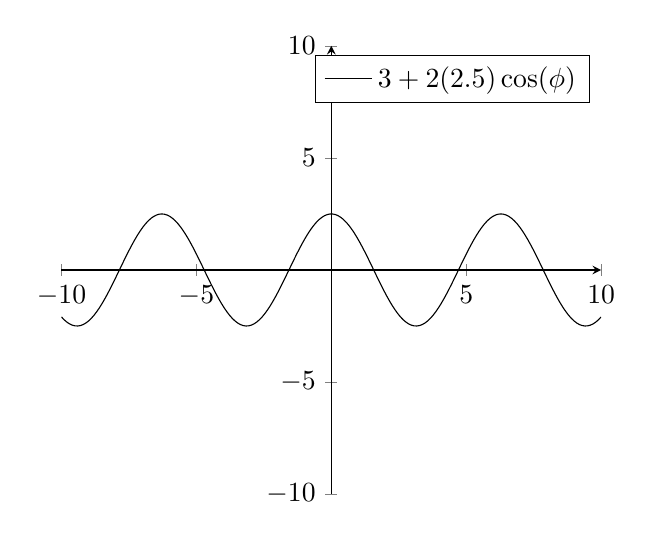
\begin{tikzpicture}
		\begin{axis}[
			xmin= -10, xmax= 10,
			ymin= -10, ymax = 10,
			axis lines = middle,
		]
			\addplot[domain=-10:10, samples=200]{ 3+2(2.5)*cos(deg(x)) };
		\legend{$3+2(2.5)\cos(\phi)$}
		\end{axis}
	\end{tikzpicture}
	\caption{Simple pgfplot for aesthetic purposes $E = 3, J = 2.5$}
	\label{}
\end{figure}
\begin{align*}
	[E_0 + 2  J\cos (\phi) ]_{\text{max}} &= E_0 + 2J \\
	[E_0 +2 J \cos (\phi)]_{\text{min}} &= E_0 - 2J  \\
\end{align*}



\section*{Problem 04} 


\begin{align*}
	\langle 1 | \hat{X} | 1 \rangle  &= 
\langle 1 | \hat{I} \hat{X} \hat{I} | 1 \rangle 
	\\ 
	&= 
\langle 1 | 
\left(\int_{0}^{L}  \mathrm{d} x \, | x \rangle \langle x | \right)
	\hat{X}
\left(\int_{0}^{L}  \mathrm{d} x' \, | x' \rangle \langle x' | \right) | 1 \rangle 
     \\ &= 
\left(\int_{0}^{L}  \mathrm{d} x \, \langle 1 | x \rangle \langle x | \right)
	\hat{X}
\left(\int_{0}^{L}  \mathrm{d} x' \, | x' \rangle \langle x' | 1 \rangle \right) 
\\ &=  
\int_{0}^{L}  \mathrm{d} x \, 
\int_{0}^{L}  \mathrm{d} x' \, 
\langle 1 | x \rangle \langle x' | 1 \rangle \langle x | \hat{X} | x' \rangle 
\\ &= 
\int_{0}^{L}  \mathrm{d} x \, 
\int_{0}^{L}  \mathrm{d} x' \, 
\langle 1 | x \rangle \langle x' | 1 \rangle x' \delta(x - x')
\\ &=
\int_{0}^{L} \mathrm{d} x \, 
\int_{0}^{L} \mathrm{d} x' \, 
\left(\sqrt{\frac{2}{L}}  \sin\left(\frac{\pi}{L}x\right) \right) 
\left(\sqrt{\frac{2}{L}}  \sin\left(\frac{\pi}{L}x'\right)\right) x' \delta(x-x')
\\ &=
\int_{0}^{L} \mathrm{d} x' \, 
\left(\sqrt{\frac{2}{L}}  \sin\left(\frac{\pi}{L}x'\right) \right) 
\left(\sqrt{\frac{2}{L}}  \sin\left(\frac{\pi}{L}x'\right)\right) x' \delta(x-x') \\
&=  
\frac{2}{L} 
\int_{0}^{L}  \mathrm{d} x' \, x' \sin^2 \left(\frac{\pi}{L}x'\right)  
\\
&= 
\frac{2}{L} \left(\frac{L}{2}\right)^2
\\
&= \frac{L}{2} 
\end{align*}

\begin{align*}
	\langle 1 | \hat{X} | 2 \rangle &= 
\int_{0}^{L} \mathrm{d} x \, 
\int_{0}^{L} \mathrm{d} x' \, 
\langle 1 | x \rangle \langle x' |  2 \rangle \langle x | \hat{X} | x' \rangle 
	\\
	&= 
\int_{0}^{L} \mathrm{d} x \, 
\int_{0}^{L} \mathrm{d} x' \, 
\left(\sqrt{\frac{2}{L}} \sin\left(\frac{\pi}{L}x\right)  \right)
\left(\sqrt{\frac{2}{L}}  \sin\left(\frac{2 \pi }{L} x' \right)\right) 
x' \delta(x- x')
	\\
	&= \frac{2}{L}
\int_{0}^{L} \mathrm{d} x' \, x' \sin\left(\frac{\pi}{L}x'\right) \sin\left(\frac{2\pi }{L}x' \right) 
	\\
	&= \frac{2}{L} \left(- \frac{8L^2}{9 \pi^2}\right) \\
	&= -\frac{16 L}{9 \pi^2} \\
\end{align*}
\begin{figure}[H]
	\centering
	\includegraphics[width=0.4\textwidth]{ss/inti01.png}
	\includegraphics[width=0.4\textwidth]{ss/inti02.png}
	\caption{ss/inti02.png}
	\label{fig:ss-inti02-png}
\end{figure}

\begin{align*}
	\langle 1 | \hat{K} | 1 \rangle  &= 
\int_{0}^{L} \mathrm{d} x' \, \langle 1 | \hat{K} | x' \rangle \langle x' | 1 \rangle 
	\\
					 & = 
					 \int_{0}^{L} \mathrm{d} x' \,
\int_{0}^{L} \mathrm{d} x  \,
\langle 1 | x \rangle \langle x |  \hat{K} | x' \rangle \langle x' | 1 \rangle 
	\\
					 & = 
					 \int_{0}^{L} \mathrm{d} x' \,
\int_{0}^{L} \mathrm{d} x  \,
\langle 1 | x \rangle \langle x |  \hat{K} | x' \rangle \langle x' | 1 \rangle 
	\\
	&= 
\frac{2}{L }\int_{0}^{L} \mathrm{d} x' \, 
\int_{0}^{L}  \mathrm{d} x \, 
\sin\left(\frac{\pi}{L}x\right) 
\langle x | \hat{K} | x' \rangle 
\sin\left(\frac{\pi}{L}x'\right) 
	\\
	&= 
\frac{2}{L }\int_{0}^{L} \mathrm{d} x' \, 
\int_{0}^{L}  \mathrm{d} x \, 
\sin\left(\frac{\pi}{L}x\right) 
\delta(x-x') \left(- i \frac{\mathrm{d} }{\mathrm{d} x'}\right)
\sin\left(\frac{\pi}{L}x'\right) 
	\\
	&= 
\frac{2}{L}
\int_{0}^{L} \mathrm{d} x' \, 
\int_{0}^{L}  \mathrm{d} x \, 
\sin\left(\frac{\pi}{L} x\right) \delta(x-x') \left(-i\right) \left(\frac{\pi}{L}\right) \cos(\frac{\pi}{L} x')
	\\
	&= 
-i \frac{2 \pi }{L^2} 
\int_{0}^{L} \mathrm{d} x' \,
\sin \left(\frac{\pi}{L} x'\right) \cos \left(\frac{\pi}{L}x'\right)
	\\ 
	&= 0 
\end{align*}

\begin{figure}[H]
	\centering
	\includegraphics[width=0.4\textwidth]{ss/inti03.png}
	\includegraphics[width=0.4\textwidth]{ss/inti04.png}
	\caption{ss/inti04.png}
	\label{fig:ss-inti04-png}
\end{figure}


\begin{align*}
	\langle 1 | \hat{K} | 2 \rangle &= 
\int_{0}^{L}  \mathrm{d}x' \,
\int_{0}^{L} \mathrm{d} x \, 
\langle 1 | x \rangle 
\langle x |  \hat{K} | x' \rangle  
\langle x' |  2\rangle 
	\\ &=  \frac{2}{L} \left(-i \frac{2\pi}{L}\right)
\int_{0}^{L}  \mathrm{d}x' \,
\int_{0}^{L} \mathrm{d} x \, 
\sin\left(\frac{\pi}{L} x\right)
\delta(x-x')
\cos\left(\frac{2\pi}{L} x'\right)
\\
&= 
-i \frac{4 \pi }{L^2} \int_{0}^{L} \mathrm{d} x' \, 
\sin\left(\frac{\pi}{L}x'\right) \cos\left(\frac{2\pi}{L}x'\right)
\\
&= 
-i \frac{4 \pi }{L^2} \left(- \frac{2L}{3 \pi }\right)\\
&= 
i \frac{8}{3L}
\\
\end{align*}

\begin{figure}[H]
	\centering
	\includegraphics[width=0.4\textwidth]{ss/inti06.png}
	\includegraphics[width=0.4\textwidth]{ss/inti07.png}
	\caption{ss/inti07.png}
	\label{fig:ss-inti07-png}
\end{figure}


\subsection*{b} 
\begin{align*}
	\langle k_1 | \hat{X} | k_1 \rangle  &= 
\langle k_1 | \hat{I} \hat{X} \hat{I}  | k_1 \rangle 
					  \\ &=
	\left(
\int_{0}^{L} \mathrm{d} x' \, \langle k_1 | x' \rangle \langle x' |  
	\right) \hat{X} 
	\left(
\int_{0}^{L}  \mathrm{d} x \, | x \rangle  \langle x | k_1 \rangle  
	\right)
	\\&= 
\int_{0}^{L} \mathrm{d} x'\,
\int_{0}^{L} \mathrm{d} x\, 
\langle k_1 | x' \rangle \langle x' | \hat{X} | x \rangle \langle x | k_1 \rangle 
	\\
	&= 
\int_{0}^{L} \mathrm{d} x'\,
\int_{0}^{L} \mathrm{d} x\, 
\langle k_1 | x' \rangle 
x \delta(x' - x)
\langle x | k_1 \rangle 
	\\
	&= 
\int_{0}^{L} \mathrm{d} x'\,
\int_{0}^{L} \mathrm{d} x\,  x 
\left(\frac{1}{\sqrt{L}  } e^{ - i k_1 x' }  \right) 
\left(\frac{1}{\sqrt{L}  } e^{  i k_1 x}  \right)  \delta(x' - x) \\
&= 
\frac{1}{L}\int_{0}^{L} \mathrm{d} x\,  x 
e^{-i k_1 x} e^{i k_1 x}
\\ 
&= 
\frac{1}{L} \int_{0}^{L} \mathrm{d} x \, x  
\\
&= 
\frac{1}{L} \left(\frac{L^2}{2}\right)
\\
&= \frac{L}{2} 
\end{align*}

\begin{align*}
	\langle k_1 | \hat{X} | k_2 \rangle &= 
	\left(
\int_{0}^{L} \mathrm{d} x'  \langle k_1 | x' \rangle \langle x' | 
	\right)
	\hat{X} 
	\left(
\int_{0}^{L}  \mathrm{d} x \, 
| x \rangle \langle x | k_2 \rangle 
	\right)
	\\
					    &= 
					    \int_{0}^{L} \mathrm{d} x'\,
\int_{0}^{L} \mathrm{d} x\, 
\langle k_1 | x' \rangle \langle x' | \hat{X} | x \rangle \langle x | k_2 \rangle 
	\\
	&= 
\frac{1}{L}
\int_{0}^{L} \mathrm{d} x' \, 
\int_{0}^{L}  \mathrm{d} x \, 
x e^{- i k_1 x' } e^{i k_2 x} \delta(x' - x)
	\\
	&= 
\frac{1}{L}
\int_{0}^{L} \mathrm{d} x \, 
x e^{i (k_2 - k_1) x} 
	\\
	&= 
\frac{1}{L}
\int_{0}^{L} \mathrm{d} x \, 
x e^{i \left(2 \frac{\pi}{L}\right) x} 
	\\ 
	&= 
	\left(\frac{1}{L} \right) \left(- \frac{i L^2}{2\pi}\right)
	\\
	&= 
- \frac{i L}{2 \pi }
	\\
\end{align*}

\begin{figure}[H]
	\centering
	\includegraphics[width=0.4\textwidth]{ss/balsal1.png}
	\includegraphics[width=0.4\textwidth]{ss/balsal2.png}
	\caption{ss/balsal2.png}
	\label{fig:ss-balsal2-png}
\end{figure}


\begin{align*}
\langle k_1 | \hat{K} | k_1 \rangle &= 
\left(
	\int_{0}^{L}  
\mathrm{d} x' \, 
\langle k_1 | x' \rangle \langle x' |  
\right)
\hat{K} 
\left(
\int_{0}^{L} \mathrm{d} x \, 
| x \rangle \langle x | k_1 \rangle 
\right)
\\	
&= 
\int_{0}^{L} \mathrm{d} x' \, 
\int_{0}^{L}  \mathrm{d} x \, 
\langle k_1 | x' \rangle 
\langle x' | \hat{K} | x \rangle 
\langle x | k_1 \rangle 
\\
&= \frac{1}{L}
\int_{0}^{L} \mathrm{d} x'
\int_{0}^{L} \mathrm{d} x 
\, 
e^{-i k_1 x'} \left(- i \delta(x' - x) \frac{\mathrm{d} }{\mathrm{d} x}\right) e^{i k_1 x }
\\
&= \frac{-i}{L}
\int_{0}^{L} \mathrm{d} x'
\int_{0}^{L} \mathrm{d} x 
\, 
e^{-i k_1 x'} \delta(x' - x) i k_1 e^{i k_1 x }
\\
&= \frac{k_1}{L}
\int_{0}^{L} \mathrm{d} x 
\, 
e^{-i k_1 x}   e^{i k_1 x }
\\
&= 
\frac{k_1}{L} \int_{0}^{L} \mathrm{d} x  
\\
&= k_1 \\
&= \frac{2\pi}{L} \\
\end{align*}


\begin{align*}
\langle k_1 | \hat{K} | k_2 \rangle &= 
\left(
	\int_{0}^{L}  
\mathrm{d} x' \, 
\langle k_1 | x' \rangle \langle x' |  
\right)
\hat{K} 
\left(
\int_{0}^{L} \mathrm{d} x \, 
| x \rangle \langle x | k_2 \rangle 
\right)
\\	
&= 
\int_{0}^{L} \mathrm{d} x' \, 
\int_{0}^{L}  \mathrm{d} x \, 
\langle k_1 | x' \rangle 
\langle x' | \hat{K} | x \rangle 
\langle x | k_2 \rangle 
\\
&= \frac{1}{L}
\int_{0}^{L} \mathrm{d} x'
\int_{0}^{L} \mathrm{d} x 
\, 
e^{-i k_1 x'} \left(- i \delta(x' - x) \frac{\mathrm{d} }{\mathrm{d} x}\right) e^{i k_2 x }
\\
&= \frac{-i}{L}
\int_{0}^{L} \mathrm{d} x'
\int_{0}^{L} \mathrm{d} x 
\, 
e^{-i k_1 x'} \delta(x' - x) i k_2 e^{i k_2 x }
\\
&= \frac{k_2}{L}
\int_{0}^{L} \mathrm{d} x 
\, 
e^{-i k_1 x}   e^{i k_2 x }
\\
&= 
\frac{k_2}{L} 
\int_{0}^{L} 
\mathrm{d} x \, e^{i \left(2 \pi / L\right) x}
\\
&= 0 
\end{align*}


\section*{Problem 05} 
\subsection{a} 
\begin{align*}
	\langle k | \hat{X} | k' \rangle &= 
	\left(
		\int_{-\infty}^{\infty} \mathrm{d} x \,  \langle k | x \rangle \langle x | 
	\right) \hat{X} 
	\left(
		\int_{-\infty}^{\infty} \mathrm{d} x' \, 
		| x' \rangle \langle x' | k' \rangle 
	\right)
	\\&= 
\int \mathrm{d} x \int \mathrm{d} x' \, 
\langle k | x \rangle \langle x | \hat{X} | x' \rangle  \langle x' | k' \rangle 
	\\
	&= 
\int \mathrm{d} x \, 
\int \mathrm{d} x ' \, 
\frac{1}{\sqrt{2\pi } } e^{-i k x} \langle x | \hat{X} | x' \rangle \frac{1}{\sqrt{2 \pi }  } e^{i k' x}
	\\
	&= 
\int \mathrm{d} x \, 
\int \mathrm{d} x ' \, 
\frac{1}{\sqrt{2\pi } } e^{-i k x} 
x ' \delta(x - x')
\frac{1}{\sqrt{2 \pi }  } e^{i k' x'}
	\\
	&= 
\int \mathrm{d} x \, 
\int \mathrm{d} x ' \, 
\frac{1}{\sqrt{2\pi } } e^{-i k x} 
 \delta(x - x')
\left( x' \frac{1}{\sqrt{2 \pi }  } e^{i k' x'} \right) 
	\\
	&= 
\int \mathrm{d} x ' \, 
\frac{1}{\sqrt{2\pi } } e^{-i k x'} 
\left( x' \frac{1}{\sqrt{2 \pi }  } e^{i k' x'} \right) 
	\\
	&= 
\int \mathrm{d} x ' \, 
\frac{1}{\sqrt{2\pi } } e^{-i k x'} 
\left( x' \frac{1}{\sqrt{2 \pi }  } e^{i k' x'} \right) 
     \\ &= \left(
	\frac{1}{\sqrt{2 \pi } } \right)^2 
	\int \mathrm{d} x' 
	\, 
	x' e^{i (k' - k )x'}
     \\ &= (-1)(-i) \left(
    \frac{1}{\sqrt{2 \pi } } \right)^2 
	\int \mathrm{d} x' 
\, \frac{\mathrm{d} }{\mathrm{d}  k }
 e^{i (k' - k )x'}
	\\
	&= 
i \frac{\mathrm{d} }{\mathrm{d} k} 
\left(
	\frac{1}{2 \pi } \int_{-\infty}^{-\infty} \mathrm{d} x\, e^{i (k' - k ) x' }
\right)
	\\  &=  
	i \frac{\mathrm{d} }{\mathrm{d} k} \delta(k' - k) = i \frac{\mathrm{d} }{\mathrm{d} k} \delta(k- k')
\end{align*}

\subsection*{b}
\begin{align*}
	\langle k | \hat{X} | f \rangle &= \int_{-\infty}^{\infty} \mathrm{d} k' \,  
\langle k | \hat{X} | k'\rangle \langle k' | f \rangle 
	\\
	 &= \int_{-\infty}^{\infty} \mathrm{d} k' \,  
	\left(
i \frac{\mathrm{d} }{\mathrm{d} k} \delta(k - k')
	\right)
\langle k' | f \rangle 
	\\
	 &= \int_{-\infty}^{\infty} \mathrm{d} k' \,  
	\left(
i \delta(k-k')\frac{\mathrm{d} }{\mathrm{d} k'}
	\right)
\langle k' | f \rangle 
	\\
	 &= \int_{-\infty}^{\infty} \mathrm{d} k' \,  
	\left(
i \delta(k-k')\frac{\mathrm{d} }{\mathrm{d} k'}
	\right)
	\left(
\int_{-\infty}^{\infty} \mathrm{d} x \, 
\frac{e^{ - i k' x}}{\sqrt{2 \pi } } f(x)
	\right)
	\\
	 &= \int_{-\infty}^{\infty} \mathrm{d} k' \,  
	\left(
i \delta(k'-k)\frac{\mathrm{d} }{\mathrm{d} k'}
	\right)
	\left(
\int_{-\infty}^{\infty} \mathrm{d} x \, 
\frac{e^{ - i k' x}}{\sqrt{2 \pi } } f(x)
	\right)
	\\
	 &=   
	\left(
i\frac{\mathrm{d} }{\mathrm{d} k}
	\right)
	\left(
\int_{-\infty}^{\infty} \mathrm{d} x \, 
\frac{e^{ - i k x}}{\sqrt{2 \pi } } f(x)
	\right)
	\\ 
	&= 
	i \frac{\mathrm{d} }{\mathrm{d} k } \tilde{f}(k)
	\\
\end{align*}












\end{document}


